% !TeX program = pdflatex
\documentclass[12pt,a4paper]{article}

% Vietnamese support (robust on Overleaf with pdfLaTeX)
\usepackage[utf8]{vietnam}

\usepackage{microtype}
\usepackage{amsmath,amssymb,amsthm,mathtools}
\usepackage{geometry}
\usepackage{graphicx}
\usepackage{tikz}
\usetikzlibrary{calc}
\usepackage{caption}
\usepackage{hyperref}
\usepackage{enumitem}

\geometry{margin=2.5cm}
\hypersetup{colorlinks=true,linkcolor=blue,urlcolor=blue,citecolor=blue}

\newtheorem{dinhly}{Định lý}
\newtheorem{mende}{Mệnh đề}
\theoremstyle{definition}
\newtheorem{dinhnghia}{Định nghĩa}
\theoremstyle{remark}
\newtheorem{nhanxet}{Nhận xét}

\DeclareMathOperator{\bd}{bd}
\DeclareMathOperator{\sgn}{sgn}

\newcommand{\R}{\mathbb{R}}
\newcommand{\trans}{^\mathsf{T}}
\newcommand{\ip}[2]{\left\langle #1,#2\right\rangle}
\newcommand{\norminf}[1]{\left\lVert #1\right\rVert_\infty}
\newcommand{\argmax}{\operatorname*{arg\,max}}

\title{Điều khiển tối ưu thời gian tuyến tính và Nguyên lý cực đại Pontryagin}
\author{NGUYỄN THỊ THẢO HIỀN}
\date{\today}

\begin{document}
\maketitle

\section{Giới thiệu}
Xét một hệ điều khiển được mô tả bởi phương trình vi phân vectơ:
\begin{equation}
\dot{x}(t)=A(t)x(t)+B(t)u(t),\qquad x(0)=x_0\in\R^n.
\label{eq:1}
\end{equation}

\begin{equation*}
\begin{aligned}
x(t)&=\begin{bmatrix}x_1(t)\\ \vdots\\ x_n(t)\end{bmatrix},
&u(t)&=\begin{bmatrix}u_1(t)\\ \vdots\\ u_m(t)\end{bmatrix},\\[4pt]
A(t)&=\begin{bmatrix}
a_{11}(t) & \cdots & a_{1n}(t)\\
\vdots & \ddots & \vdots\\
a_{n1}(t) & \cdots & a_{nn}(t)
\end{bmatrix},
&B(t)&=\begin{bmatrix}
b_{11}(t) & \cdots & b_{1m}(t)\\
\vdots & \ddots & \vdots\\
b_{n1}(t) & \cdots & b_{nm}(t)
\end{bmatrix}.
\end{aligned}
\end{equation*}

Trong đó
\begin{itemize}[leftmargin=2.2em]
  \item $x(t)$: là vectơ trạng thái (state vector),
  \item $u(t)$: vectơ điều khiển/đầu vào.
\end{itemize}

\textbf{Giả định về tính khả tích:} Giả sử các phần tử của $A(t)$, $B(t)$ là các hàm khả tích trên bất kỳ khoảng thời gian hữu hạn. Điều này đảm bảo các nghiệm của phương trình vi phân tồn tại và duy nhất trong những khoảng thời gian đó.

\textbf{Tập các điều khiển được chấp nhận:}
\begin{equation}
\Delta\;\coloneqq\;\Bigl\{u(\cdot)=(u_1(\cdot),\ldots,u_m(\cdot))\trans:\ |u_i(t)|\le 1,\ i=1,\ldots,m\Bigr\}.
\label{eq:2}
\end{equation}
Trong phần còn lại, ta dùng ký hiệu $\mathcal{U}\equiv\Delta$.

\subsection{Bài toán điều khiển tối ưu thời gian}
\noindent\textbf{Bài toán điều khiển:}
Cho trước một điểm mục tiêu $x_1\in\R^n$.\\
Tìm một tín hiệu điều khiển $u(t)\in\Delta$ sao cho hệ thống đạt đến trạng thái $x(t_1)=x_1$.\\
Tối thiểu hóa thời gian $t_1$ để đạt được mục tiêu đó.

\par\noindent $\rightarrow$ Đây là một bài toán điều khiển tối ưu thời gian. Mục tiêu bài toán là tìm luật điều khiển tối ưu $u^*(t)\in\Delta$ đưa hệ thống từ trạng thái ban đầu $x_0$ đến điểm trạng thái đích $x_1$ trong thời gian $t_1$ ngắn nhất.

\par\noindent Từ lý thuyết phương trình vi phân, nghiệm của \eqref{eq:1} có thể được viết là:
\begin{equation}
\tag{3}\label{eq:sol-3}
x(t;u)=X(t)x_0+X(t)\int_{0}^{t}X^{-1}(\tau)B(\tau)u(\tau)\,d\tau.
\end{equation}
Trong đó $X(t)$ là ma trận nghiệm chính của hệ thuần nhất $\dot X(t)=A(t)X(t)$, $X(0)=I$ (với $I$ là ma trận đơn vị).

Việc nắm được tập trạng thái có thể đạt được tại thời điểm $t$ sẽ cung cấp một mô tả đầy đủ về các điểm có thể chạm tới trong khoảng thời gian đến $t$ và cho phép tái cấu trúc bài toán điều khiển về dạng: tối thiểu hóa $t_1$ để $x_1\in\mathcal{A}(t_1)$, với $\mathcal{A}(t)\coloneqq\{x(t;u):u(\cdot)\in\Delta\}$.

Nói cách khác, ta xét bài toán tối ưu thời gian:
\begin{equation}
\tag{4}\label{eq:tstar}
t^*\;\coloneqq\;\inf\Bigl\{t_1>0\ \big|\ \exists\,u(\cdot)\in\mathcal{U}\ \text{sao cho}\ x(t_1; x_0, u)=x_1\Bigr\}.
\end{equation}
Mục tiêu là tìm điều khiển tối ưu $u^*(\cdot)$ đưa hệ từ trạng thái ban đầu $x_0$ đến trạng thái đích $x_1$ trong thời gian tối thiểu $t^*$.

\section{Nghiệm của hệ và phép biến đổi}
Để phân tích khả năng tiếp cận các trạng thái mục tiêu, ta xét khái niệm
\emph{tập trạng thái có thể đạt được} tại thời điểm $t$, ký hiệu là $\mathcal{A}(t)$, được định nghĩa là tập bao gồm tất cả các điểm $x\in\R^n$ mà hệ thống có thể đạt tới đúng tại thời điểm $t$ khi sử dụng một tín hiệu điều khiển hợp lệ $u(\cdot)\in\Delta$:
\begin{equation*}
\mathcal{A}(t)=\{x(t;u):\ u(\cdot)\in\Delta\}.
\end{equation*}

Việc hiểu rõ cấu trúc của $\mathcal{A}(t)$ cung cấp một mô tả đầy đủ về phạm vi hoạt động của hệ thống theo thời gian.
Đối với bài toán điều khiển thời gian tối ưu tuyến tính, điều khiển tối ưu sẽ tồn tại nếu điểm mục tiêu $x_1$ có thể đạt được trong một khoảng thời gian nào đó; điều kiện này liên hệ chặt chẽ với tính \emph{khả điều khiển} (controllability) của hệ.

Từ bây giờ, ta giả sử tồn tại điều khiển tối ưu $u^*$ với thời gian tối thiểu $t^*$, và xét bài toán đặc trưng hoá $u^*$. Ở đây, để trình bày gọn đúng tinh thần tài liệu gốc, ta trước hết xét trường hợp một biến điều khiển $m=1$ (khi đó $B(t)$ là ma trận $n\times 1$); trường hợp tổng quát chỉ khác về ký hiệu.

Gọi $X(t)$ là ma trận nghiệm chính của hệ thuần nhất
\begin{equation}
\tag{5}\label{eq:X}
\dot{X}(t)=A(t)X(t),\qquad X(0)=I.
\end{equation}
trong đó $I$ là ma trận đơn vị (xem, ví dụ, \cite{hermes} cho công thức nghiệm theo ma trận chuyển tiếp).

Từ lý thuyết phương trình vi phân, nghiệm của \eqref{eq:1} có thể viết dưới dạng biến thiên hằng số:
\begin{equation}
\tag{6}\label{eq:sol}
x(t)=X(t)x_0+\int_0^t X(t)X^{-1}(\tau)B(\tau)u(\tau)\,d\tau.
\end{equation}

\subsection{Đặt biến để đơn giản hóa}
Đặt
\begin{equation}
\tag{7}\label{eq:C}
C(t)\;\coloneqq\;X^{-1}(t)B(t)\in\R^{n\times m}.
\end{equation}
Trong trường hợp $m=1$, $C(t)$ là một vectơ trong $\R^n$; theo ký hiệu thường gặp trong tài liệu gốc có thể viết
\[
C(t)=y(t)=\bigl(y_1(t),\ldots,y_n(t)\bigr)\trans.
\]
Để đơn giản hóa các phương trình, hai biến mới được định nghĩa:
\begin{itemize}[leftmargin=2.2em]
  \item $y(t)$: đại lượng liên kết ma trận nghiệm chính với ma trận đầu vào,
  \item $y_1(t)$: trạng thái mục tiêu sau biến đổi (tóm tắt mục tiêu cuối cùng $x_1$ so với trạng thái ban đầu $x_0$ trong hệ biến đổi).
\end{itemize}

Từ \eqref{eq:sol} ta có
\begin{equation}
\tag{8}\label{eq:Xinvx}
X^{-1}(t)x(t)=x_0+\int_0^t C(\tau)u(\tau)\,d\tau.
\end{equation}
Do đó, đặt
\begin{equation}
\tag{9}\label{eq:y-y1}
y(t)\;\coloneqq\;\int_0^t C(\tau)u(\tau)\,d\tau\in\R^n,
\qquad
y_1(t)\;\coloneqq\;X^{-1}(t)x_1-x_0\in\R^n.
\end{equation}
Khi đó điều kiện $x(t)=x_1$ tương đương với
\begin{equation}
\tag{10}\label{eq:reach-cond}
y(t)=y_1(t).
\end{equation}

Đặc biệt, tại thời điểm tối ưu $t^*$ với điều khiển tối ưu $u^*$, đặt gọn
\[
y_1\;\coloneqq\;y_1(t^*)=X^{-1}(t^*)x_1-x_0\in\R^n,
\]
thì từ \eqref{eq:y-y1} suy ra đúng như trong tài liệu gốc:
\begin{equation*}
y_1=\int_{0}^{t^*}C(\tau)u^*(\tau)\,d\tau\qquad (m=1:\ C(\tau)=y(\tau)).
\end{equation*}

\section{Định nghĩa và Tính chất của $R(t)$}

\noindent\textbf{Định nghĩa.} $R(t)$ là tập các trạng thái có thể đạt được tại thời điểm $t$ trong không gian biến đổi (tức là tập các giá trị của tích phân vectơ khi ta thay đổi điều khiển $u(\tau)$ hợp lệ trong $\Delta$).

Trong trường hợp minh hoạ thường gặp $m=1$ (một biến điều khiển), ta có thể viết $C(\tau)=y(\tau)\in\R^n$ và
\begin{equation}
\tag{11}\label{eq:R}
R(t)=\left\{\int_0^t y(\tau)u(\tau)\,d\tau:\ u(\cdot)\in\Delta\right\}
=\left\{\left(\int_0^t y_1(\tau)u(\tau)\,d\tau,\ \int_0^t y_2(\tau)u(\tau)\,d\tau,\ \ldots,\ \int_0^t y_n(\tau)u(\tau)\,d\tau\right)\trans:\ u(\cdot)\in\Delta\right\}.
\end{equation}

\noindent (Với trường hợp tổng quát $m\ge 1$, biểu thức tương ứng là $R(t)=\{\int_0^t C(\tau)u(\tau)\,d\tau:\ u(\cdot)\in\Delta\}$, trong đó $C(\tau)\in\R^{n\times m}$.)

\noindent\textbf{Tính chất.} Tập $R(t)$ được chứng minh là:
\begin{itemize}[leftmargin=2.2em]
  \item \textbf{đóng} (closed),
  \item \textbf{bị chặn} (bounded),
  \item \textbf{lồi} (convex).
\end{itemize}
Tính lồi là then chốt vì cho phép áp dụng các định lý hình học mạnh (đặc biệt là định lý siêu phẳng đỡ) để suy ra các điều kiện cực đại kiểu Pontryagin.

\subsection{Mối quan hệ giữa $\mathcal{A}(t)$ và $R(t)$}
Gọi $\mathcal{A}(t)$ là tập trạng thái có thể đạt được tại thời điểm $t$ trong không gian gốc:
\[\mathcal{A}(t)\coloneqq\{x(t;u):u(\cdot)\in\Delta\}.\]
Từ công thức nghiệm \eqref{eq:sol} và phép biến đổi $y(t)=\int_0^t C(\tau)u(\tau)\,d\tau$ suy ra ánh xạ tuyến tính qua ma trận nghiệm chính $X(t)$:
\begin{equation}
\tag{12}\label{eq:A-from-R}
\mathcal{A}(t)=X(t)\bigl[x_0+R(t)\bigr]=\bigl\{X(t)[x_0+y]:\ y\in R(t)\bigr\}.
\end{equation}
Ngược lại,
\begin{equation}
R(t)=X^{-1}(t)\,\mathcal{A}(t)-x_0.
\label{eq:R-from-A}
\end{equation}
Các công thức này cho thấy $R(t)$ và $\mathcal{A}(t)$ chứa cùng thông tin, chỉ khác nhau bởi phép biến đổi tuyến tính qua $X(t)$ và tịnh tiến bởi $x_0$.

\section{Điều kiện tối ưu về thời gian $t^*$}
\textbf{Điều kiện tối ưu về thời gian ($t^*$): Khi nào thì một thời điểm $t^*$ là nhỏ nhất:}
\par\noindent
$x_1$: điểm mục tiêu\\
$y_1$: điểm mục tiêu tương ứng trong không gian $R$.

\par\noindent
Đặt tập trạng thái có thể đạt được tại thời điểm $t$ trong không gian gốc là
\[\mathcal{A}(t)\;\coloneqq\;\{x(t;u):u(\cdot)\in\mathcal{U}\}.\]
Vì $x_1\in\mathcal{A}(t^*)$, ta có $y_1(t^*)\in R(t^*)$, và rõ ràng $t^*$ là thời điểm nhỏ nhất mà $y_1(t)\in R(t)$ (nếu không, ta có $x_1\in\mathcal{A}(\bar t)$ với $\bar t<t^*$; giả thiết này là mâu thuẫn).

Do đó:
\begin{equation}
\tag{13}\label{eq:y1inR}
y_1(t^*)\in R(t^*).
\end{equation}

Hơn nữa, thời gian tối thiểu $t^*$ là thời điểm đầu tiên mà điểm mục tiêu $y_1$ \emph{chạm} vào tập $R(t)$; vì vậy $y_1(t^*)$ phải nằm trên \emph{biên} của $R(t^*)$ (không nằm trong nội của tập):
\begin{equation}
\tag{14}\label{eq:boundary}
y_1(t^*)\in \bd R(t^*).
\end{equation}

% (Tài liệu gốc đánh số đây là Hình 2)
\setcounter{figure}{1}
\begin{figure}[h]
\centering
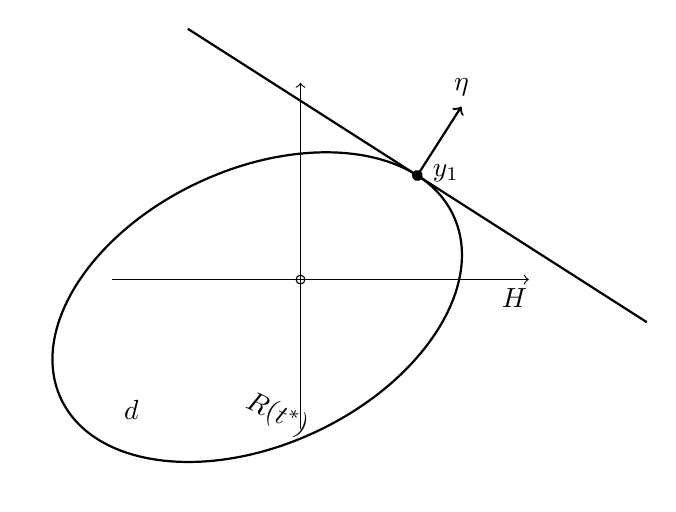
\begin{tikzpicture}[scale=1]
  % axes (cross at origin) -- giống hình scan
  \draw[->] (-2.4,0) -- (2.9,0);
  \draw[->] (0,-1.9) -- (0,2.5);
  \draw (0,0) circle (1.6pt);

  % parameters for a "scan-like" tilted ellipse
  % NOTE: avoid \a, \b macro names (can clash with Vietnamese accent macros)
  \pgfmathsetmacro{\ellipseA}{2.75}
  \pgfmathsetmacro{\ellipseB}{1.75}
  \pgfmathsetmacro{\ellipseRot}{25} % tilt of ellipse
  \pgfmathsetmacro{\thetaParam}{22} % param angle (controls y1 location)

  % ellipse, tangency, supporting line H and outward normal eta
  \begin{scope}[shift={(-0.55,-0.35)}, rotate=\ellipseRot]
    \draw[thick] (0,0) ellipse ({\ellipseA} and {\ellipseB});

    % point y1 on ellipse boundary
    \coordinate (Y1) at ({\ellipseA*cos(\thetaParam)},{\ellipseB*sin(\thetaParam)});

    % tangent direction at Y1 in local ellipse coords
    \pgfmathsetmacro{\tangx}{-\ellipseA*sin(\thetaParam)}
    \pgfmathsetmacro{\tangy}{ \ellipseB*cos(\thetaParam)}
    \draw[thick] ($(Y1)+(-1.8*\tangx,-1.8*\tangy)$) -- ($(Y1)+(1.8*\tangx,1.8*\tangy)$);

    % outward normal direction (scaled)
    \pgfmathsetmacro{\normx}{cos(\thetaParam)/\ellipseA}
    \pgfmathsetmacro{\normy}{sin(\thetaParam)/\ellipseB}
    \draw[->,thick] (Y1) -- ++(2.6*\normx,2.6*\normy) node[above] {$\eta$};

    % mark y1
    \fill (Y1) circle (2pt);
    \node[anchor=west] at ($(Y1)+(0.08,0.00)$) {$y_1$};

    % labels inside ellipse
    \node[rotate=-\ellipseRot] at (-0.35,-1.35) {$R(t^*)$};
  \end{scope}

  % label H near lower part of tangent line
  \node[anchor=west] at ($(Y1)+(0.95,-1.55)$) {$H$};

  % small "d" marker
  \node at (-2.15,-1.65) {$d$};
\end{tikzpicture}
\captionsetup{labelsep=none}
\caption{}
\label{fig:2}
\end{figure}

Tại $t=0$, $R(t)=\{0\}$; khi thời gian tăng lên, $R(t)$ phát triển và cuối cùng giao với điểm $y_1$. Bài toán trở thành tìm thời điểm đầu tiên $t^*$ mà tại đó $R(t)$ giao với $y_1$. Chúng ta kỳ vọng (như được chỉ ra trong Hermes) rằng tiếp xúc đầu tiên xảy ra khi $R(t^*)$ chỉ chạm vào $y_1$, hay $y_1$ phải thuộc biên của $R(t^*)$.

\section{Định lý siêu phẳng đỡ và Điều kiện Cực đại}
\textbf{Định lý Siêu phẳng Đỡ và Điều kiện Cực đại:}
\begin{itemize}[leftmargin=2.2em]
  \item Định lý siêu phẳng hỗ trợ phát biểu rằng tại một điểm trên biên của một tập lồi ($y_1$ trên biên của $R(t^*)$), tồn tại ít nhất một siêu phẳng đi qua điểm đó mà toàn bộ tập lồi nằm về một phía của siêu phẳng.
\end{itemize}

Theo Định lý Siêu phẳng Đỡ, tồn tại một siêu phẳng không tầm thường $H$ (có pháp tuyến hướng ra ngoài là $\eta$) hỗ trợ $R(t^*)$ tại $y_1$, nghĩa là khi chiếu tất cả các điểm $y\in R(t^*)$ lên phương $\eta$, điểm $y_1$ cho giá trị lớn nhất (cực đại):
\begin{equation}
\eta\trans y_1\;\ge\;\eta\trans y,\qquad \forall\,y\in R(t^*),\ \eta\neq 0.
\label{eq:support}
\end{equation}

\par\noindent\textbf{Trong đó:}
\begin{itemize}[leftmargin=2.2em]
  \item $H$: siêu phẳng (hyperplane).
  \item $\eta$: vectơ pháp tuyến (normal vector) của siêu phẳng, khác $0$.
  \item $\eta\trans y$: biểu diễn phép nhân vô hướng (dot product) hoặc phép chiếu lên phương $\eta$.
\end{itemize}

\subsection{Bất đẳng thức tích phân và điều kiện cực đại Pontryagin}
Vì mọi $y\in R(t^*)$ có dạng $y=\int_0^{t^*} C(t)u(t)\,dt$, từ \eqref{eq:support} suy ra
\begin{equation}
\eta\trans y_1
\;=\;\max_{u(\cdot)\in\mathcal{U}}\ \int_0^{t^*} \eta\trans C(t)u(t)\,dt.
\label{eq:max-integral}
\end{equation}
Điều này dẫn đến điều kiện rằng $u^*(t)$ phải cực đại hóa biểu thức dưới dấu tích phân tại hầu hết mọi thời điểm $t$.

Đặc biệt, trong trường hợp một điều khiển vô hướng ($m=1$) và viết $y(t)\coloneqq C(t)\in\R^n$ (với $y(t)=(y_1(t),\ldots,y_n(t))\trans$), điều kiện cực đại ở trên có thể viết tương đương dưới dạng bất đẳng thức tích phân sau (Điều kiện Cực đại Pontryagin):
\begin{equation}
\eta\trans\!\left(\int_{0}^{t^*} y(\tau)u^*(\tau)\,d\tau\right)
\;\ge\;
\eta\trans\!\left(\int_{0}^{t^*} y(\tau)u(\tau)\,d\tau\right),
\qquad \forall\,u(\cdot)\in\Delta.
\label{eq:pmp-int-vec}
\end{equation}

Biến đổi (với $\eta=(\eta_1,\ldots,\eta_n)\trans$), ta được
\begin{equation}
\int_{0}^{t^*}\bigl(\eta_1y_1(\tau)+\eta_2y_2(\tau)+\cdots+\eta_ny_n(\tau)\bigr)\,\bigl(u^*(\tau)-u(\tau)\bigr)\,d\tau\;\ge\;0,
\qquad \forall\,u(\cdot)\in\Delta.
\label{eq:pmp-int-sum}
\end{equation}

Hay gọn hơn:
\begin{equation}
\int_{0}^{t^*}\bigl(\eta\trans y(\tau)\bigr)\,\bigl(u^*(\tau)-u(\tau)\bigr)\,d\tau\;\ge\;0,
\qquad \forall\,u(\cdot)\in\Delta.
\label{eq:pmp-int-compact}
\end{equation}

\textbf{Kết quả của Nguyên lý cực đại Pontryagin áp dụng cho bài toán điều khiển thời gian tối ưu tuyến tính.}

Điều này chỉ xảy ra nếu
\[
u^*(\tau)=\sgn\bigl(\eta\trans y(\tau)\bigr),\qquad \tau\in(0,t^*).
\]
Trong đó:
\[
\sgn(x)=\begin{cases}
+1, & \text{nếu } x>0,\\
-1, & \text{nếu } x<0,\\
\text{không xác định}, & \text{nếu } x=0.
\end{cases}
\]
\begin{itemize}[leftmargin=2.2em]
  \item Nếu biểu thức $x$ dương, điều khiển $u^*(t)$ nhận giá trị cực đại dương $(+1)$.
  \item Nếu biểu thức $x$ âm, điều khiển $u^*(t)$ nhận giá trị cực đại âm $(-1)$.
  \item Trường hợp biểu thức bằng $0$ $(x=0)$ là trường hợp đặc biệt (điểm chuyển mạch), nơi $u^*(t)$ có thể không xác định hoặc chuyển dấu.
\end{itemize}

Do đó, chứng minh được định lý sau, một trường hợp đặc biệt của Nguyên lý cực đại Pontryagin.

\par\noindent\textbf{Định lý 1:}
Nếu $u^*$ là một điều khiển tối ưu bất kỳ dịch chuyển từ $x_0$ đến $x_1$ trong thời gian tối thiểu $t^*$ thì tồn tại một vectơ $\eta\in\R^n$, $\eta\neq 0$ sao cho:
\begin{equation}
u^*(t)=\sgn\bigl(\eta\trans y(t)\bigr)=\sgn\bigl(\eta\trans X^{-1}(t)B(t)\bigr),\qquad t\in[0,t^*].
\tag{4}
\end{equation}

Trong trường hợp tổng quát ($m$ biến điều khiển), với $u^*(t)=(u_1^*(t),\ldots,u_m^*(t))\trans$, có:
\begin{equation}
u_i^*(t)=\sgn\Bigl(\bigl[\eta\trans X^{-1}(t)B(t)\bigr]_i\Bigr),
\qquad i=1,\ldots,m,\ \ t\in[0,t^*],
\tag{5}
\end{equation}
trong đó $[\cdot]_i$ là thành phần thứ $i$ của vectơ. Từ đây, ta viết \eqref{eq:max-integral} tương đương dưới dạng vectơ:
\begin{equation}
u^*(t)=\sgn\Bigl(\bigl(\eta\trans X^{-1}(t)B(t)\bigr)\trans\Bigr),\qquad t\in[0,t^*].
\tag{6}
\end{equation}
trong đó $\sgn(\cdot)$ tác động theo từng thành phần (component-wise) khi đối số là một vectơ.

\section{Mối liên hệ giữa điều khiển tối ưu với phương trình Adjoint}

\subsection{Phương trình Adjoint (phương trình biến liên hợp)}
Tài liệu định nghĩa hàm biến liên hợp (costate variable) $\psi(t)$ là
\begin{equation}
\psi(t)\;\coloneqq\;\eta\trans X^{-1}(t).
\label{eq:psi-def}
\end{equation}
Hàm này phải tuân theo một phương trình vi phân riêng biệt gọi là Phương trình Adjoint. Thật vậy, do
\[\frac{d}{dt}X^{-1}(t)=-X^{-1}(t)A(t),\]
ta suy ra
\begin{equation}
\dot{\psi}(t)=-\psi(t)A(t).
\label{eq:adjoint}
\end{equation}

Đặt định lý ở Mục 5 dưới dạng thường được phát biểu bằng cách lưu ý rằng hàm
\[\psi(t)=\eta\trans X^{-1}(t)\]
là nghiệm của phương trình Adjoint (phương trình biến liên hợp)
\[\dot\psi(t)=-\psi(t)A(t),\qquad \text{với điều kiện ban đầu }\psi(0)=\eta\trans.\]

Thật vậy, từ $\psi(t)=\eta\trans X^{-1}(t)$ suy ra $\psi(t)X(t)=\eta\trans$ (hằng theo $t$). Lấy đạo hàm, ta có
\begin{align*}
0
&=\frac{d}{dt}\bigl(\eta\trans\bigr)
=\frac{d}{dt}\bigl(\psi(t)X(t)\bigr)
=\dot\psi(t)X(t)+\psi(t)\dot X(t)\\
&=\dot\psi(t)X(t)+\psi(t)A(t)X(t)
=\bigl(\dot\psi(t)+\psi(t)A(t)\bigr)X(t).
\end{align*}
Vì $X(t)$ khả nghịch, suy ra $\dot\psi(t)=-\psi(t)A(t)$.

Do đó, các công thức \textup{(4)}--\textup{(6)} có thể viết lại gọn dưới dạng
\begin{equation}
u^*(t)=\sgn\Bigl(\bigl(\psi(t)B(t)\bigr)\trans\Bigr),\qquad 0\le t\le t^*.
\tag{7}
\end{equation}

\par\noindent\textbf{Trong đó:}
\begin{itemize}[leftmargin=2.2em]
  \item $\psi(t)$: vectơ hàng biến liên hợp.
\end{itemize}

\subsection{Hamiltonian $H(\psi,x,u)$ và Nguyên lý Cực đại}
Hamiltonian là một hàm vô hướng kết hợp trạng thái $x$, biến liên hợp $\psi$ và điều khiển $u$:
\begin{equation}
H(\psi,x,u)\;\coloneqq\;\psi A(t)x+\psi B(t)u.
\tag{11}
\label{eq:hamiltonian}
\end{equation}
Tương đương, $H(\psi,x,u)=\psi\bigl(A(t)x+B(t)u\bigr)$, nhưng cách viết \eqref{eq:hamiltonian} làm rõ rằng đây là một tích vô hướng giữa vectơ hàng $\psi$ với véctơ động lực học $\dot x$.

Nếu định nghĩa Hamiltonian bởi
\[H(\psi,x,u)=\psi\bigl(A(t)x+B(t)u\bigr),\]
thì điều khiển tối ưu \textup{(7)} thỏa mãn điều kiện cực đại:
\[
H\bigl(\psi(t),x(t),u^*(t)\bigr)=\max_{u\in U} H\bigl(\psi(t),x(t),u\bigr),
\qquad t\in[0,t^*],
\]
trong đó $U=[-1,1]^m$ (tương ứng với các ràng buộc trong $\Delta$).

Nguyên lý Cực đại phát biểu rằng điều khiển tối ưu $u^*(t)$ phải là giá trị điều khiển làm cho Hamiltonian đạt giá trị cực đại tại mọi thời điểm $t\in[0,t^*]$:
\begin{equation}
H\bigl(\psi(t),x(t),u^*(t)\bigr)=\max_{u\in U} H\bigl(\psi(t),x(t),u\bigr),\qquad t\in[0,t^*].
\tag{12}
\label{eq:pmp-hamiltonian}
\end{equation}
với $U=[-1,1]^m$.

\subsection{Điều khiển \emph{bang-bang} là gì?}
Trong bài toán bị chặn biên độ $U=[-1,1]^m$, hạng phụ thuộc điều khiển trong Hamiltonian là tuyến tính theo $u$:
\[H(\psi,x,u)=\psi A(t)x+\bigl(\psi B(t)\bigr)u.\]
Vì thế, để cực đại hóa theo $u$ tại mỗi thời điểm, nghiệm tối ưu (khi không rơi vào trường hợp suy biến) sẽ chọn ngay các giá trị \emph{biên} của miền điều khiển.
Điều khiển như vậy được gọi là \textbf{bang-bang}: mỗi thành phần $u_i^*(t)$ chỉ nhận các giá trị $+1$ hoặc $-1$ (gần như mọi $t$), và chỉ \emph{chuyển} giữa $+1$ và $-1$ tại các \textbf{thời điểm chuyển mạch} (switching times) khi biểu thức quyết định đổi dấu.

\begin{itemize}[leftmargin=2.2em]
  \item Do tập điều khiển $\Delta$ bị giới hạn biên độ (ví dụ $[-1,1]$), điều kiện cực đại hóa Hamiltonian dẫn đến việc $u^*(t)$ phải nhảy giữa các giá trị biên.
\end{itemize}

Trong trường hợp một điều khiển vô hướng ($m=1$), khi đó $u(t)\in[-1,1]$ và $\psi(t)B(t)$ là một số thực. Khi đó:
\begin{itemize}[label=+,leftmargin=2.2em]
  \item Nếu $\psi(t)B(t)>0$ thì $u^*(t)=+1$.
  \item Nếu $\psi(t)B(t)<0$ thì $u^*(t)=-1$.
\end{itemize}
Đây chính là điều khiển bang-bang. Khi hàm \textbf{switching function}
\[\sigma(t)\coloneqq \psi(t)B(t)\]
đi qua điểm $0$, các nghiệm của phương trình $\sigma(t)=0$ chính là các \textbf{thời điểm chuyển mạch} mà tại đó điều khiển bang-bang thay đổi trạng thái (từ $+1$ sang $-1$ hoặc ngược lại).

Cụ thể, nếu đặt
\[\Phi(t)\coloneqq \eta\trans X^{-1}(t)B(t)\in\R^{1\times m},\]
thì dạng điều khiển đã thu được ở Mục 5 chính là
\[u_i^*(t)=\sgn\bigl(\,[\Phi(t)]_i\,\bigr),\qquad i=1,\ldots,m,\ t\in[0,t^*],\]
và khi $[\Phi(t)]_i=0$ thì $u_i^*(t)$ có thể không xác định tức thời (điểm chuyển mạch) hoặc có nhiều lựa chọn tương đương.

\begin{thebibliography}{9}
\bibitem{hermes}
H. Hermes, \emph{Time-Optimal Control}, ghi chú/bài giảng kinh điển về điều khiển tối ưu thời gian tuyến tính.
\end{thebibliography}

\end{document}
